% -----------------------------------------------
% Template for ISMIR Papers
% 2017 version, based on previous ISMIR templates

% Requirements :
% * 6+n page length maximum
% * 4MB maximum file size
% * Copyright note must appear in the bottom left corner of first page
% * Clearer statement about citing own work in anonymized submission
% (see conference website for additional details)
% -----------------------------------------------

\documentclass{article}
\usepackage{ismir,amsmath,cite,url}
\usepackage{graphicx}
\usepackage{color}


% Title.
% ------
\title{Paper Template For ISMIR \conferenceyear}

% Note: Please do NOT use \thanks or a \footnote in any of the author markup

% Single address
% To use with only one author or several with the same address
% ---------------
%\oneauthor
% {Names should be omitted for double-blind reviewing}
% {Affiliations should be omitted for double-blind reviewing}

% Two addresses
% --------------
%\twoauthors
%  {First author} {School \\ Department}
%  {Second author} {Company \\ Address}

%% To make customize author list in Creative Common license, uncomment and customize the next line
%  \def\authorname{First Author, Second Author}


% Three addresses
% --------------
\threeauthors
  {First Author} {Affiliation1 \\ {\tt author1@ismir.edu}}
  {Second Author} {\bf Retain these fake authors in\\\bf submission to preserve the formatting}
  {Third Author} {Affiliation3 \\ {\tt author3@ismir.edu}}

%% To make customize author list in Creative Common license, uncomment and customize the next line
%  \def\authorname{First Author, Second Author, Third Author}

% Four or more addresses
% OR alternative format for large number of co-authors
% ------------
%\multauthor
%{First author$^1$ \hspace{1cm} Second author$^1$ \hspace{1cm} Third author$^2$} { \bfseries{Fourth author$^3$ \hspace{1cm} Fifth author$^2$ \hspace{1cm} Sixth author$^1$}\\
%  $^1$ Department of Computer Science, University , Country\\
%$^2$ International Laboratories, City, Country\\
%$^3$  Company, Address\\
%{\tt\small CorrespondenceAuthor@ismir.edu, PossibleOtherAuthor@ismir.edu}
%}
%\def\authorname{First author, Second author, Third author, Fourth author, Fifth author, Sixth author}


\sloppy % please retain sloppy command for improved formatting

\begin{document}

%
\maketitle
%
\begin{abstract}
In this paper we aim at automatically identify patterns that are intrinsic for a given musical genre. Algorithms doing this effectively could be used, for instance, to improve current music recommendation systems. To this end, we applied two symbolic music algorithms capable of dealing with polyphonic music on a Midi file dataset with genre annotations. We experimented on the classification results with several settings involving both patterns of rhythmic information only and patterns containing tonic information, as well. Our best settings give significantly better results than a random classifier. 
\end{abstract}
%
\section{Introduction}\label{sec:introduction}

The identification of repeated patterns in a collection of songs had been studied in multiple areas of the music information retrieval field, initially for identifying a song in a big collection querying only with a sequence of notes, but also recent works focused on the analysis of the importance of repeated patterns for specific genres \cite{boot,koops,odekerken,forth}.

In this paper we apply a more general approach for identifying important patterns for musical genres by processing with automatic pattern recognition algorithms a big collection of Midi files of a wide variety of genres. The identification of this patterns will allow to analyze different musical genres by a computational approach, also to improve recommendation systems and the evaluation of other methods by comparing with this results.

For this task we used the Lakh dataset \cite{raffel} of midi files which is mapped to the Million Song Dataset (MSD) \cite{Bertin-Mahieux2011} and the top-MAGD dataset \cite{Schindler:3} of genre annotations over the Million Song Dataset.

In order to identify the different patterns for each song we use 2 algorithms for automatic patterns detection. The first algorithm used is SIA \cite{doi:10.1076/jnmr.31.4.321.14162} based on geometric representation in euclidean space for identifying patterns on polyphonic music, the other algorithm is P2 \cite{Ukkonen:2} also based on geometric representation but designed to efficiently finding a sequence of notes in a song. Therefore the time complexity of P2 is $O(mn\log n)$ where m is the number of notes to query and n the number of notes in the song. While the for SIA the order is $O(kn^2\log_2 n)$ where n is the number of notes and k the dimension.

We use two different approaches for evaluating the quality of the extracted patterns by the different algorithms. First we only extract rhythmic patterns and we compare them with the dataset developed by Vurkaç \cite{vurkac}, (available from UCI learning repository \cite{Lichman:2013}). This dataset contains 10800 bars in onset notation were each bar is annotated with the clave direction, we will refer to it as the Clave dataset. The second approach used to evaluate the algorithms consisted in extracting patterns with tonic information and using them to classify the songs by genre.

(Related Works: ...
Multiple works had studied the importance of identifying repeated patterns on musical works.)

The rest of this paper is organized as follows. In section 2 presents the evaluation of the algorithms only using rhythm information, while the section 3 presents the results of classification the songs by genre using the extracted patterns. Finally the conclusions and future work are presented in section 3. 

\section{Rhythmic patterns}

\begin{table}
 \begin{center}
 \begin{tabular}{|l|l|l|}
  \hline
  Name & Compactness & Temporal Density \\
  \hline
  SiaRhythm1 & 0.7 &0.025 \\
  \hline
  SiaRhythm2 & 0.4 & 0.025 \\
  \hline
  SiaRhythm3 & 0.7 & 0.25 \\
  \hline
  SiaRhythm4 & 0.4 & 0.25 \\
  \hline
 \end{tabular}
\end{center}
 \caption{SIA algorithm thresholds for discarding patterns}
 \label{siarhythm}
\end{table}


\begin{table}
 \begin{center}
 \begin{tabular}{|l|l|l|p{1.2cm}|}
  \hline
  Name & Length (notes) & Offset (notes) & Similarity  \\
  \hline
  P2rhythm3 & 3 & 3 & 0.9 \\
  \hline
  P2rhythm4 & 4 & 3 & 0.9 \\
  \hline
  P2rhythm5 & 5 & 3 & 0.9 \\
  \hline
  P2rhythm10 & 10 & 5 & 0.6 \\
  \hline
  P2rhythm15 & 15 & 5 & 0.6 \\
  \hline
  P2rhythm15b & 15 & 3 & 0.6 \\
  \hline
  P2rhythm20 & 20 & 3 & 0.6 \\
  \hline
  P2rhythm25 & 25 & 3 & 0.6 \\
  \hline
 \end{tabular}
\end{center}
 \caption{P2 algorithm values for selecting query sequences and similarity threshold for discarding patterns}
 \label{p2rhythm}
\end{table}


Using different settings for each algorithm we extracted different patterns for each song. For the SIA algorithm we discarded the patterns that were below this three thresholds:
\begin{itemize}
\item Compactness: The length of the pattern according to the length of the song
\item Temporal Density: A pattern with more notes than other of the same length will have a higher density
\item Length: All patterns with less than 3 notes were discarded
\end{itemize}

In \tabref{siarhythm} are specified the different combination of thresholds from Compactness and Temporal Density.

The algorithm P2 allows to find a given sequence of notes in a song, for this algorithm we used as input each section of the same song with different lengths and a given overlap between the sections. The algorithm returns a measure of similarity for each retrieved match between 0 and 1. The different measures of length and offset are specified in \tabref{p2rhythm}, a different similarity threshold where use for each configuration which is specified in \tabref{p2rhythm} as well. 

\subsection{Evaluation of extracted rhythmic patterns}

In order to know which setting for each algorithm works better we compare the results with the Clave Dataset which is the biggest public dataset with rhythmic information that we could find. This dataset was manually double-blind annotated which information of the presence of a clave and its direction, we take this as a ground truth of rhythmic patterns (discarding the patterns labeled as incoherent).

As it was mentioned above in the Clave Dataset the bars are in onset notation which means that is represented as a sequence of 0 and 1’s of length 16 where 1 indicates the onset of a note. While the patterns extracted from the MIDI files contains the information of the “tick” of each note. In order to compare them we need to find a common representation.

\begin{enumerate}
\item Example of a pattern on Clave Dataset:  \begin{verbatim}1 0 0 1 0 0 1 0 0 0 1 0 1 0 0 0\end{verbatim}
\item Example of pattern extracted from a MIDI file: \begin{verbatim}0  545  682  818\end{verbatim}
\end{enumerate}

Since the MIDI files could have different values of ticks per quarter note the first step was to convert all the patterns to the same value of ticks per quarter note, this information is present in the header of the MIDI file and the value used for the conversion was 6 which is very low but is only for the comparison with the Clave Dataset patterns. 
The patterns of Clave Dataset were converted first to indexes and then used the same concept of ticks per quarter note to representing it, so the values after the conversion for the previous examples are:

\begin{enumerate}
\item \begin{verbatim}0|4|9|15|18\end{verbatim}  ticks per quarter note was 4
\item \begin{verbatim}0|3|4 \end{verbatim} ticks per quarter note was 480
\end{enumerate}

\subsubsection{Results}

\begin{figure}
 \centerline{\framebox{
 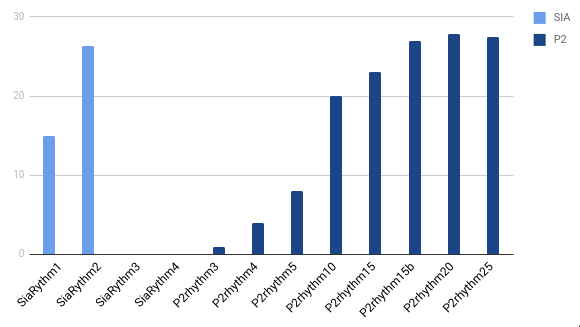
\includegraphics[width=\columnwidth]{figs/rhythm_coverage.png}}}
 \caption{Percentage of coverage of the different patters extracted on Clave rhythm patterns dataset}
 \label{rhythmcover}
\end{figure}

\begin{figure}
 \centerline{\framebox{
 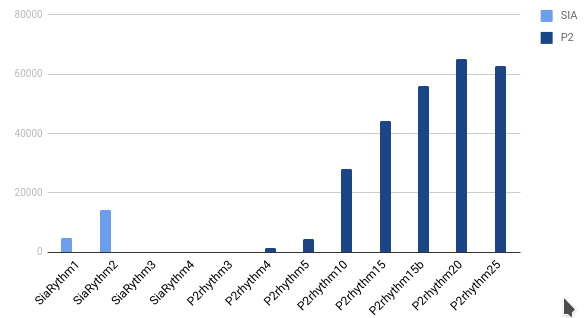
\includegraphics[width=\columnwidth]{figs/rhythm_count.png}}}
 \caption{Percentage of coverage of the different patters extracted on Clave rhythm patterns dataset}
 \label{rhythmcount}
\end{figure}

According to the comparisons on \figref{rhythmcover} there is a big difference between the results of the different settings for each algorithm. Algorithm SIA with the setting SiaRhythm2 gets 26\% of coverage over the Clave Dataset while with the algorithm P2 with the setting P2Rhythm20 gets 27\%. Using the settings SiaRhythm2 a good coverage is achieved, in part this is because it contains larger patterns which the other settings couldn’t retrieve.

\subsection{Distinctive rhythmic patterns by genre}

Since there are many patterns that are very common in all genres we will use the TF-IDF measure to get the 5 most distinctive patterns for each genre. (Once the patterns are identified we could reconvert them to the original MIDI representation)

Jazz patterns:
\begin{itemize}
\item \begin{verbatim} 0|1|3|4|7|9|12|13|15|16|19\end{verbatim}
\item \begin{verbatim} 0|1|3|4|7|9|12|13|15|16|19|21 \end{verbatim}
\item \begin{verbatim} 0|1|3|4|7|9|12|13|16|19|21 \end{verbatim}
\item \begin{verbatim} 0|3|7|9|12|15 \end{verbatim}
\item \begin{verbatim} 0|1|3|4|9|12|13|15|16|21 \end{verbatim}
\end{itemize}

The matrix on \figref{confusiongenres} shows the number of common patterns between the different genres if we only select the top 500 patterns sorted by the TF-IDF measure over the patterns extracted by SiaRhythm2. This shows that there is almost no intersection between the most distinctive patterns on each genre, the only exception is Reggae, Folk and Blues where there are not enough patterns extracted. 

\begin{figure}
 \centerline{\framebox{
 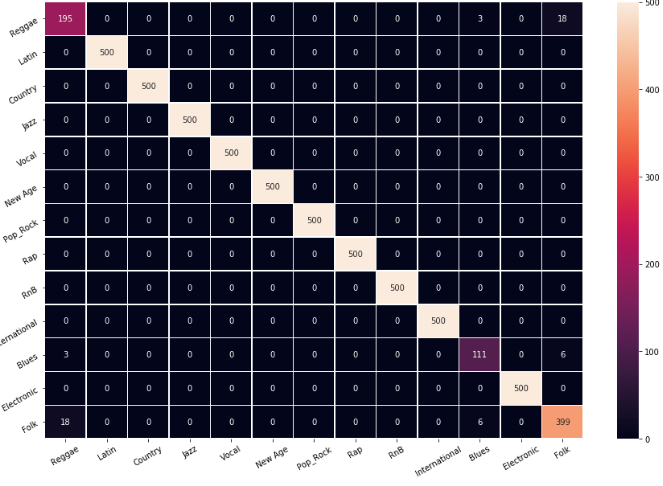
\includegraphics[width=\columnwidth]{figs/confusiongenres.png}}}
 \caption{Number of common patterns between the genres.}
 \label{confusiongenres}
\end{figure}



\section{Patterns with tonic information}


\begin{table}
 \begin{center}
 \begin{tabular}{|l|l|l|}
  \hline
  Name & Compactness & Temporal Density \\
  \hline
  SiaTonic1 & 0.7 & 0.05 \\
  \hline
  SiaTonic2 & 0.4 & 0.05 \\
  \hline
  SiaTonic3 & 0.4 & 0.25 \\
  \hline
  SiaTonic4 & 0.7 & 0.25 \\
  \hline
 \end{tabular}
\end{center}
 \caption{SIA algorithm thresholds for discarding patterns with tonic information}
 \label{siatonic}
\end{table}


\begin{table}
 \begin{center}
 \begin{tabular}{|l|l|l|l|}
  \hline
  Name & Length (notes) & Offset (notes) & Similarity  \\
  \hline
  P2tonic3 & 3 & 2 & 0.9 \\
  \hline
  P2tonic4 & 4 & 2 & 0.9 \\
  \hline
  P2tonic5 & 5 & 3 & 0.5 \\
  \hline
  P2tonic8 & 8 & 3 & 0.5 \\
  \hline
  P2tonic10 & 10 & 3 & 0.5 \\
  \hline
  P2tonic15 & 15 & 3 & 0.5 \\
  \hline
  P2tonic20 & 20 & 3 & 0.5 \\
  \hline
  P2tonic25 & 25 & 3 & 0.5 \\
  \hline
 \end{tabular}
\end{center}
 \caption{P2 algorithm values for selecting query sequences and similarity threshold for discarding patterns with tonic information}
 \label{p2tonic}
\end{table}

After identifying the best configuration for the algorithms to extract rhythmic patters we have processed again the MIDI files with both algorithms but this time with tonic information. Different settings for each algorithm were tested. In \tabref{siatonic} we show the thresholds for discarding patterns on each configuration for SIA algorithm, and in \tabref{p2tonic} we show the values used to query the for each song and the similarity threshold for discarding patterns.

Since there is no big enough public dataset of patterns with tonic information the evaluation of the extracted patters is done by measuring the performance on classification of the songs by genre. If the patters extracted show a good performance in the classification it means  they are able to capture the important information that refers to the genre in a song.  

The patters extracted with each algorithm will be combined with the set of rhythmic patterns extracted with SiaRhythm2, which was explained in the last section. We showed that this set of patterns has a better trade off between coverage and number of patterns and we think this good trade off will be important in the classification because keeps only the relevant information necessary to classify the songs. But we will evaluate if combining with only rhythmic patterns will improve the performance because it's possible that the same information is already covered by other patters.

Something that has to be noted for this classification is that the annotations are very unbalanced, because the category \textit{Pop\_Rock} contains about 60\% of the dataset.

\subsection{Classification of genre with extracted patterns}

For comparing the performance of the different settings first we classify only with the patterns with tonic information and then we combined them with the patterns extracted using SiaRhythm2. 

In order to classify the following approach is used: each pattern is represented as a string where each note is represented as \verb=(position|tone)=, for example this is a valid pattern: \begin{verbatim} (0|57)(3|59)(10|56) \end{verbatim}

For the classification we create a binary matrix where the columns correspond to the different patterns found and the rows to the different songs. For each position of the matrix if the pattern was found for the corresponding song then will have the value: 1, otherwise 0 is present. This matrix is the input to the classification algorithm, for this task we are using Logistic Regression and weights of the classes are automatically balanced by the algorithm. The scikit-learn implementation is used for this task \cite{scikit-learn}.

From the result on \tabref{tonic_results} of this evaluation is clear that with P2 algorithm we get much better performance than with SIA, also we can see how larger sequences get better accuracy but after 20 notes there are no enough patterns retrieved. Is also interesting to note that when more patterns are found then the classification performance is better but after some point there is no much improvement. 

In \tabref{tonic_rhythm_results} the results of combining the patterns with tonic information with the patterns on SiaRhythm2 for the classification are shown, in this case there is no significant improvement which could be explained because the patterns in SiaRhythm2 are only 14291 and it doesn't add more information contrary as we thought initially.  

\begin{table}
 \begin{center}
 \begin{tabular}{|l|c|c|c|p{1.2cm}|}
  \hline
  Name & Accuracy & Recall& Precision& \#patterns\\
  \hline
  SiaTonic1 & 39.47 & 69.54 & 67.98 & 130394 \\
  \hline
  SiaTonic3 & 37.62 & 69.16 & 67.47 & 81547 \\
  \hline
  SiaTonic4 & 36.05 & 68.89 & 67.14 & 54890  \\
  \hline
  SiaTonic2 & 40.85 & 69.87 & 68.39 & 236586 \\
  \hline
  P2tonic5 & 61.24 & \textbf{73.59} & \textbf{71.39} & 2763773 \\
  \hline
  P2tonic4 & 56.36 & 71.51 & 71.42 & 2083114 \\
  \hline
  P2tonic3 & 44.20 & 65.99 & 68.78 & 1002232 \\
  \hline
  P2tonic15 & \textbf{62.09} & 73.34 & 69.60 & 2671666 \\
  \hline
  P2tonic8 & 61.90 & 73.39 & 70.44 & 3560508 \\
  \hline
  P2tonic10 & 61.82 & 73.27 & 70.19 & 3693755 \\
  \hline
 \end{tabular}
\end{center}
 \caption{SIA and P2 algorithm performance of classifying songs by genre}
 \label{tonic_results}
\end{table}


\begin{table}
 \begin{center}
 \begin{tabular}{|l|c|c|c|}
  \hline
  Name & Accuracy & Recall& Precision \\
  \hline
  SiaTonic1 & 38.07 & 69.45 & 67.70 \\
  \hline
  SiaTonic3 & 36.59 & 68.92 & 67.05 \\
  \hline
  SiaTonic4 & 34.92 & 71.78 & 66.74 \\
  \hline
  SiaTonic2 & 39.55 & 69.69 & 68.15 \\
  \hline
  P2tonic5 & 61.24 & 73.84 & 71.68 \\
  \hline
  P2tonic4 & 56.10 & 71.69 & 71.58  \\
  \hline
  P2tonic3 & 44.40 & 66.35 & 69.20  \\
  \hline
  P2tonic15 & 62.07 & 73.55 & 69.77  \\
  \hline
  P2tonic8 & 61.97 & 73.69 & 70.69 \\
  \hline
  P2tonic10 & 61.88 & 73.54 & 70.49 \\
  \hline
 \end{tabular}
\end{center}
 \caption{SIA and P2 algorithm performance of classifying songs by genre by combining rhythmic and tonic patterns}
 \label{tonic_rhythm_results}
\end{table}

\section{Conclusions and future work}

Even if the algorithms were design for different tasks, we expected to have similar results by calling multiple times the algorithm P2 with different sections but having the advantage of computing the patterns faster. The results shown on sections 2 and 3 are very different for both algorithms but this doesn't contradict our initial idea, since there might exist a different combination of the thresholds that give similar results for both algorithms. As the goal of this work was to find the best set of patters that describes the different genres we didn't focus on finding a similar result for the algorithms.

We found the results of the classification very interesting but also we see this patters as a good source to combine with other sources to improve other methods, e.g for a multi-modal approach like on \cite{oramas2017multi} could be extended with the extracted patterns. 

Other algorithms for patterns detection could be analyzed in the same way by applying the same methodology, for example the algorithms based on DTW could be an interesting alternative to combine patterns in a better way.

Also it would be interesting to apply an unsupervised method for clustering the patters to analyze the relations between the different genres of even between the artists.

Therefore we want to make this set of patterns public to promote further research like the already mentioned and others as well.

Finally we would like to mention that other dataset of labels of genres over the MSD could be used with the same methodology, for this purpose all the code used is available on line \footnote{Github repository with the code here}.




--------

Other ideas that can be in the introduction:

The identification of repeated patterns in a collection of songs has been applied to analyze the similarity between this songs and has been proofed the importance of the patters for classifying songs in some genres. REF XX. Also, the concept of genre can be understand as a way of grouping songs by different aspects. In this paper we present a way of identifying important patterns for different genres by detecting the repetition of notes in different songs annotated with genre. 

Genre classification of songs has been very studied in MIR, but the publication of the Lakh dataset mapped with the Million Song Dataset allows for the first time the analysis of a big corpus of midi files with annotation of genre, which will allow to study genres from different new perspectives and in a bigger scale.

There is not enough ground truth for comparing the results of the extracted patterns, this is mentioned on MIREX challenge Discovery of Repeated Themes \& Sections as the main reason why there is not a challenge on inter-opus pattern discovery. 

% For bibtex users:
\bibliography{ISMIRtemplate}

% For non bibtex users:
%\begin{thebibliography}{citations}
%
%\bibitem {Author:00}
%E. Author.
%``The Title of the Conference Paper,''
%{\it Proceedings of the International Symposium
%on Music Information Retrieval}, pp.~000--111, 2000.
%
%\bibitem{Someone:10}
%A. Someone, B. Someone, and C. Someone.
%``The Title of the Journal Paper,''
%{\it Journal of New Music Research},
%Vol.~A, No.~B, pp.~111--222, 2010.
%
%\bibitem{Someone:04} X. Someone and Y. Someone. {\it Title of the Book},
%    Editorial Acme, Porto, 2012.
%
%\end{thebibliography}

\end{document}
